\chapter{\uppercase{Neutrino Oscillation in the PROSPECT AD}}

\section{Data Set}
\begin{figure}[H]
	\centering
	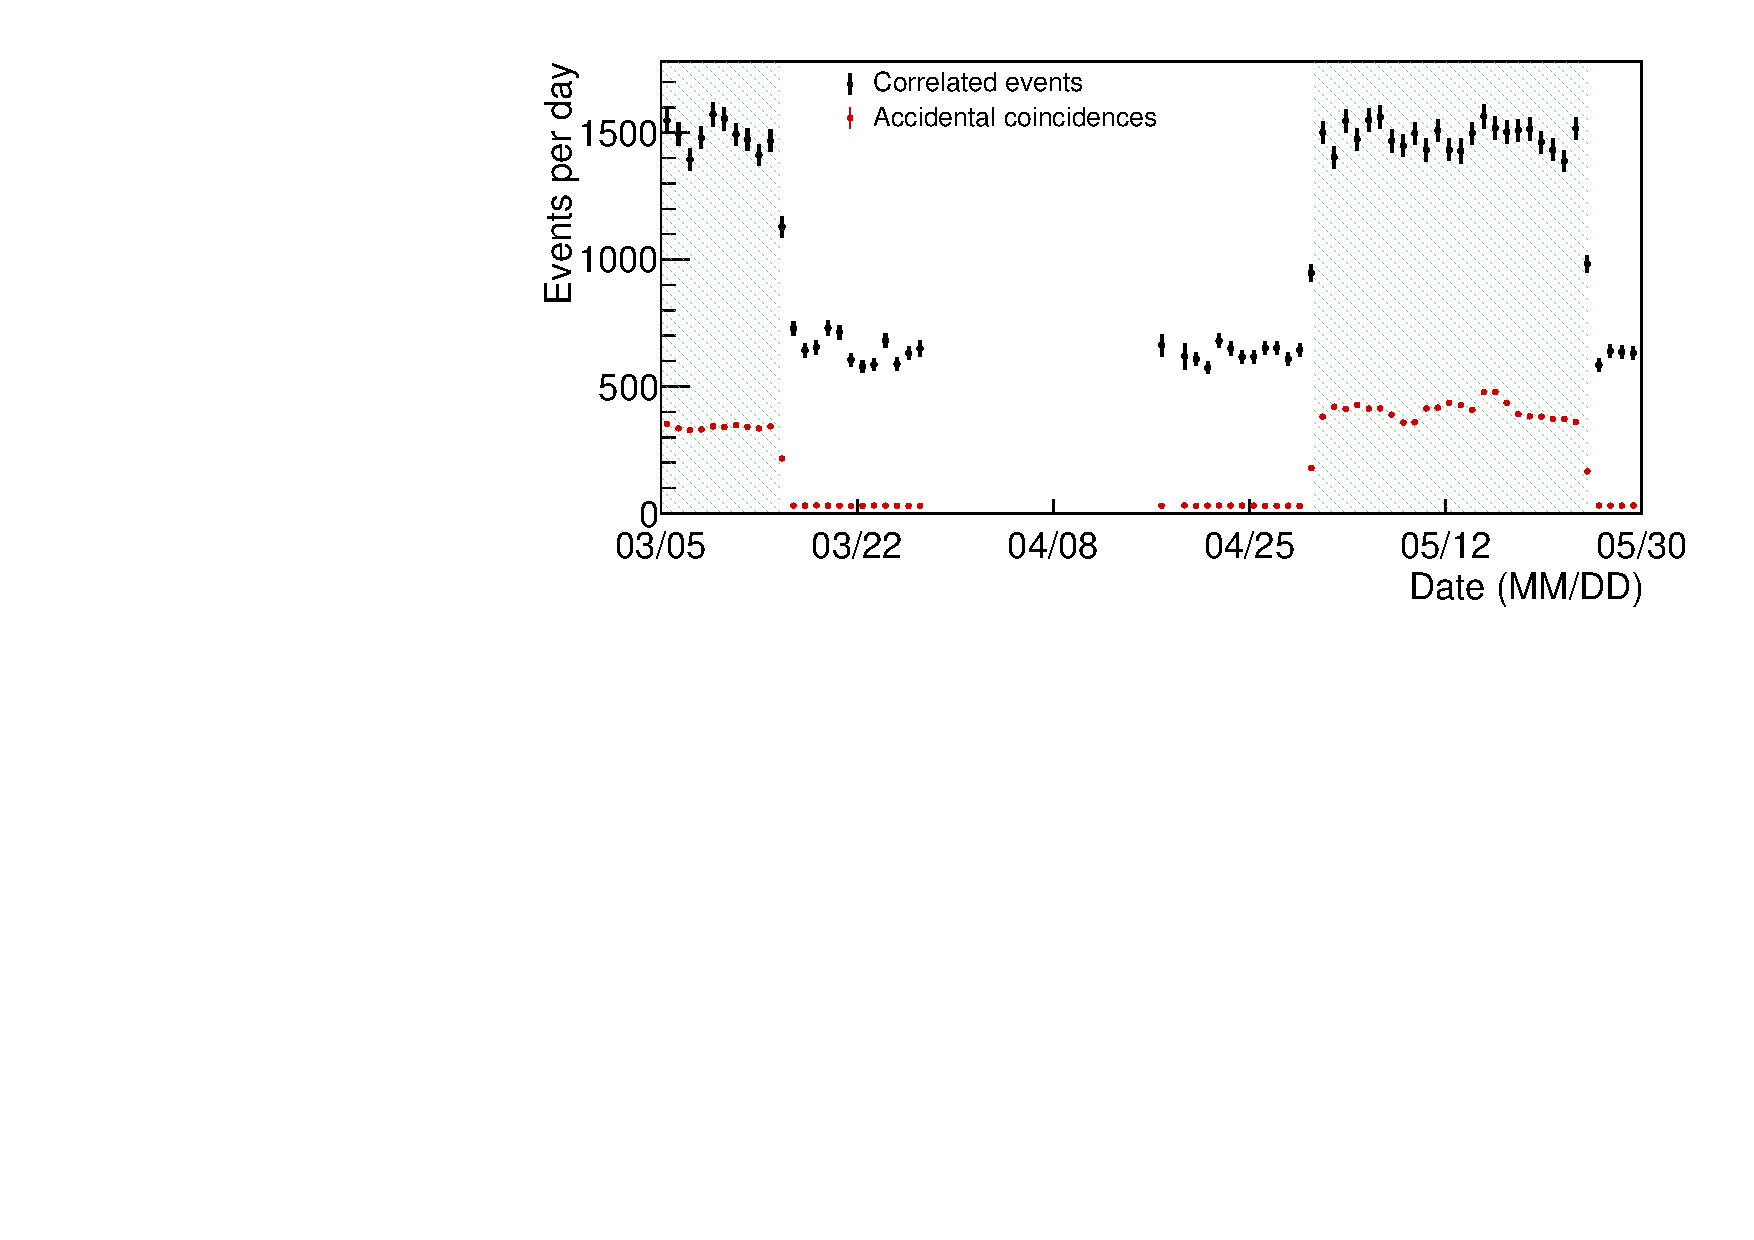
\includegraphics[width=0.7\linewidth]{tex/7-oscillation-images/EvtRates}
	\caption{}
	\label{fig:evtrates}
\end{figure}


\section{IBD Event Selection}

Cuts: 
\begin{itemize}
	\item Prompt PSD
	\item Delay PSD
	\item Delay energy
	\item Prompt-delay time coincidence
	\item Prompt-delay distance
	\item Shower veto
	\item Fiducialization
\end{itemize}

\noindent Background:
\begin{itemize}
	\item Cosmogenics
	\item Atmospheric correction
	\item Background subtraction
\end{itemize}

\begin{figure}[H]
	\centering
	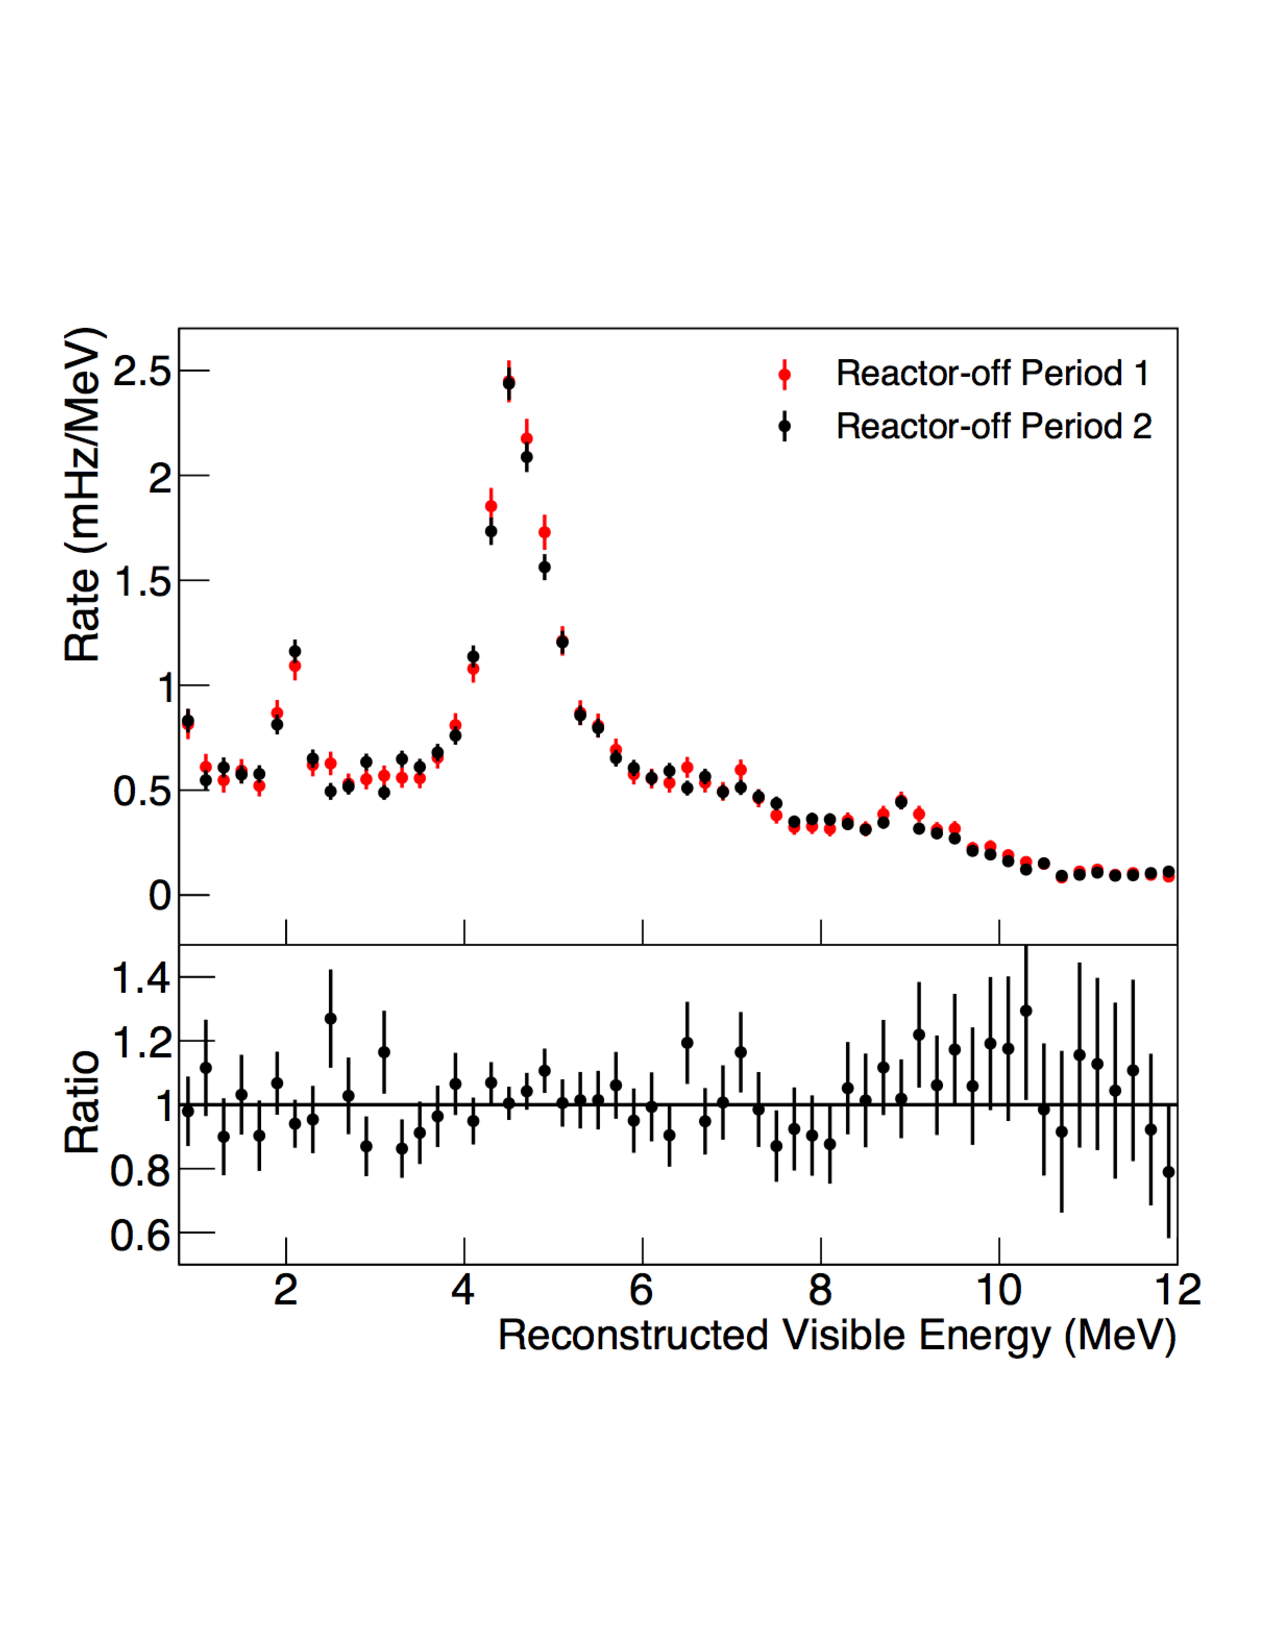
\includegraphics[width=0.7\linewidth]{tex/7-oscillation-images/RxOffSpectrum}
	\caption{}
	\label{fig:rxoffspectrum}
\end{figure}



\begin{figure}[H]
	\centering
	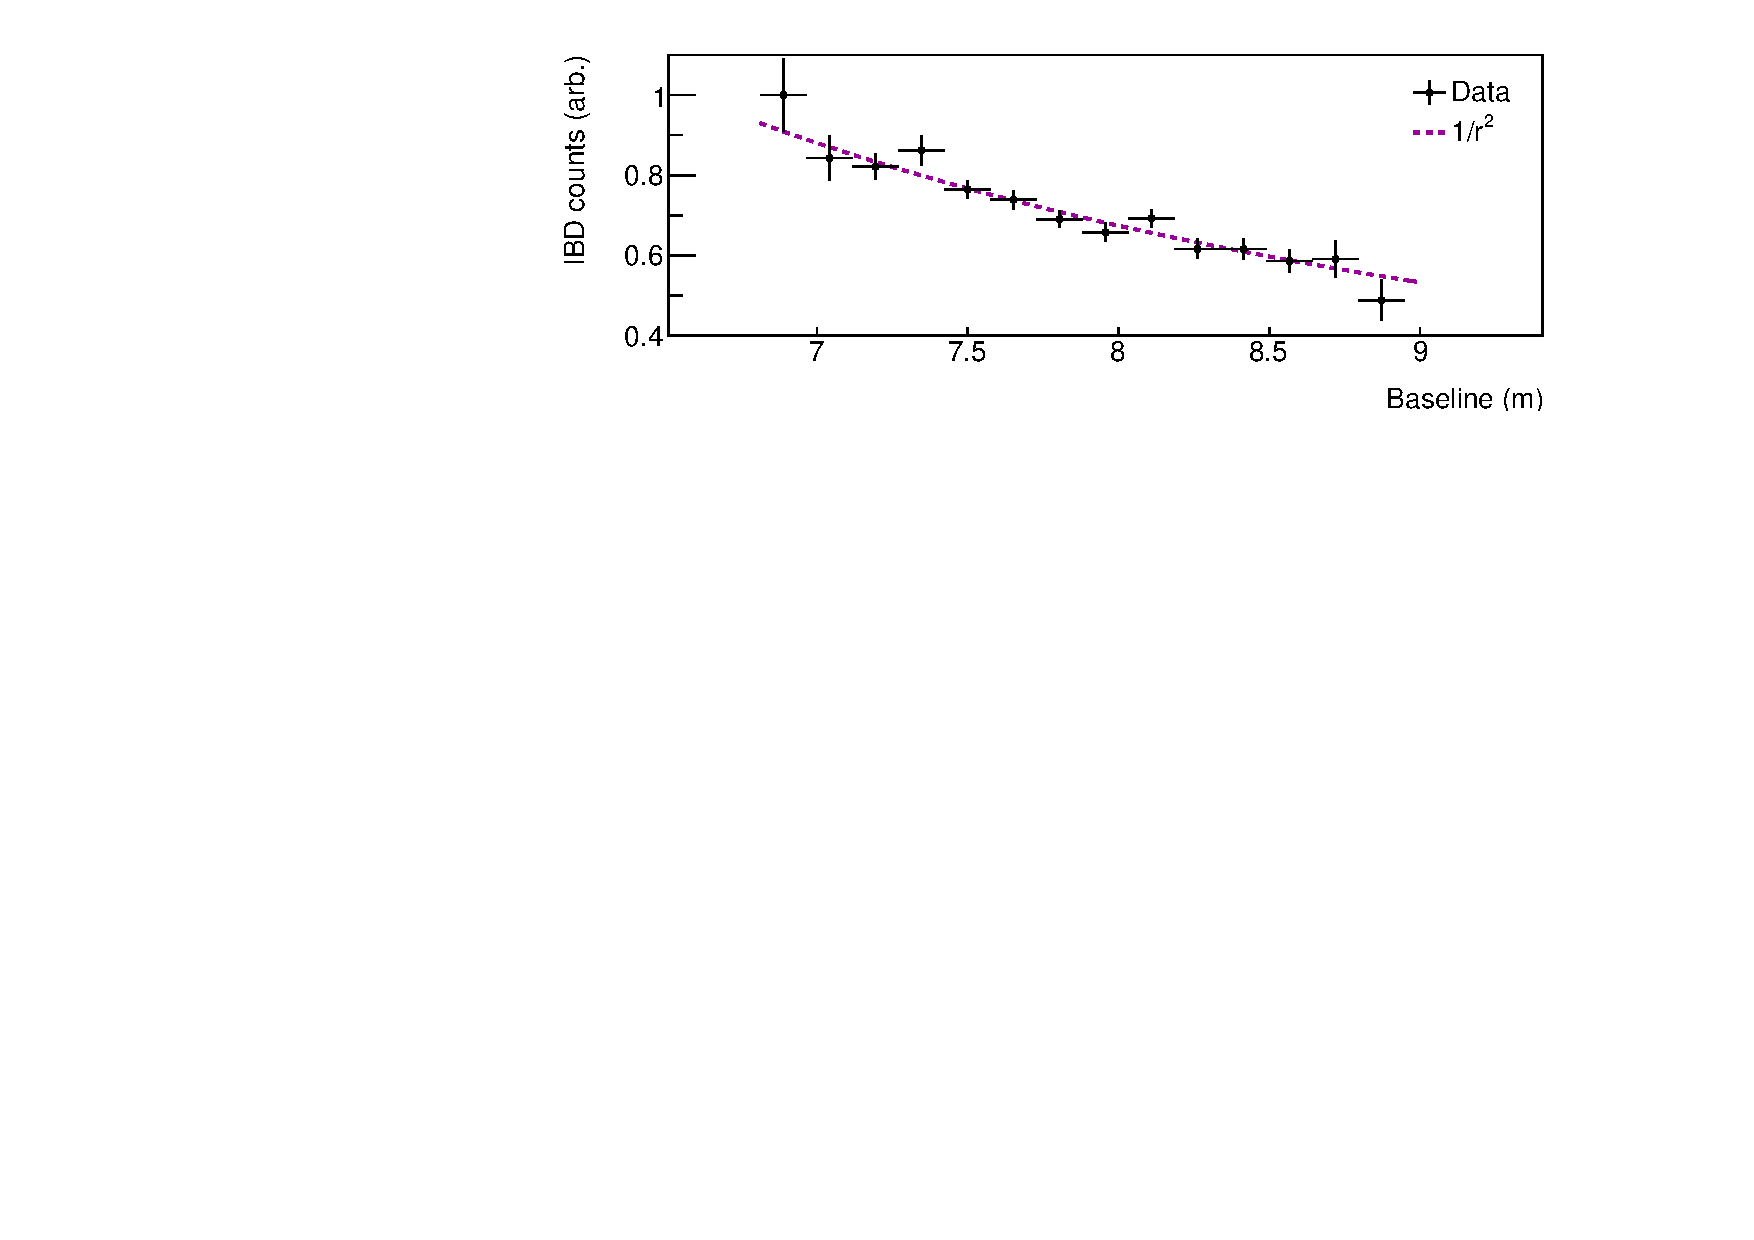
\includegraphics[width=0.7\linewidth]{tex/7-oscillation-images/IBDvsBaseline}
	\caption{}
	\label{fig:ibdvsbaseline}
\end{figure}



\section{Oscillation Results}

\begin{figure}[H]
	\centering
	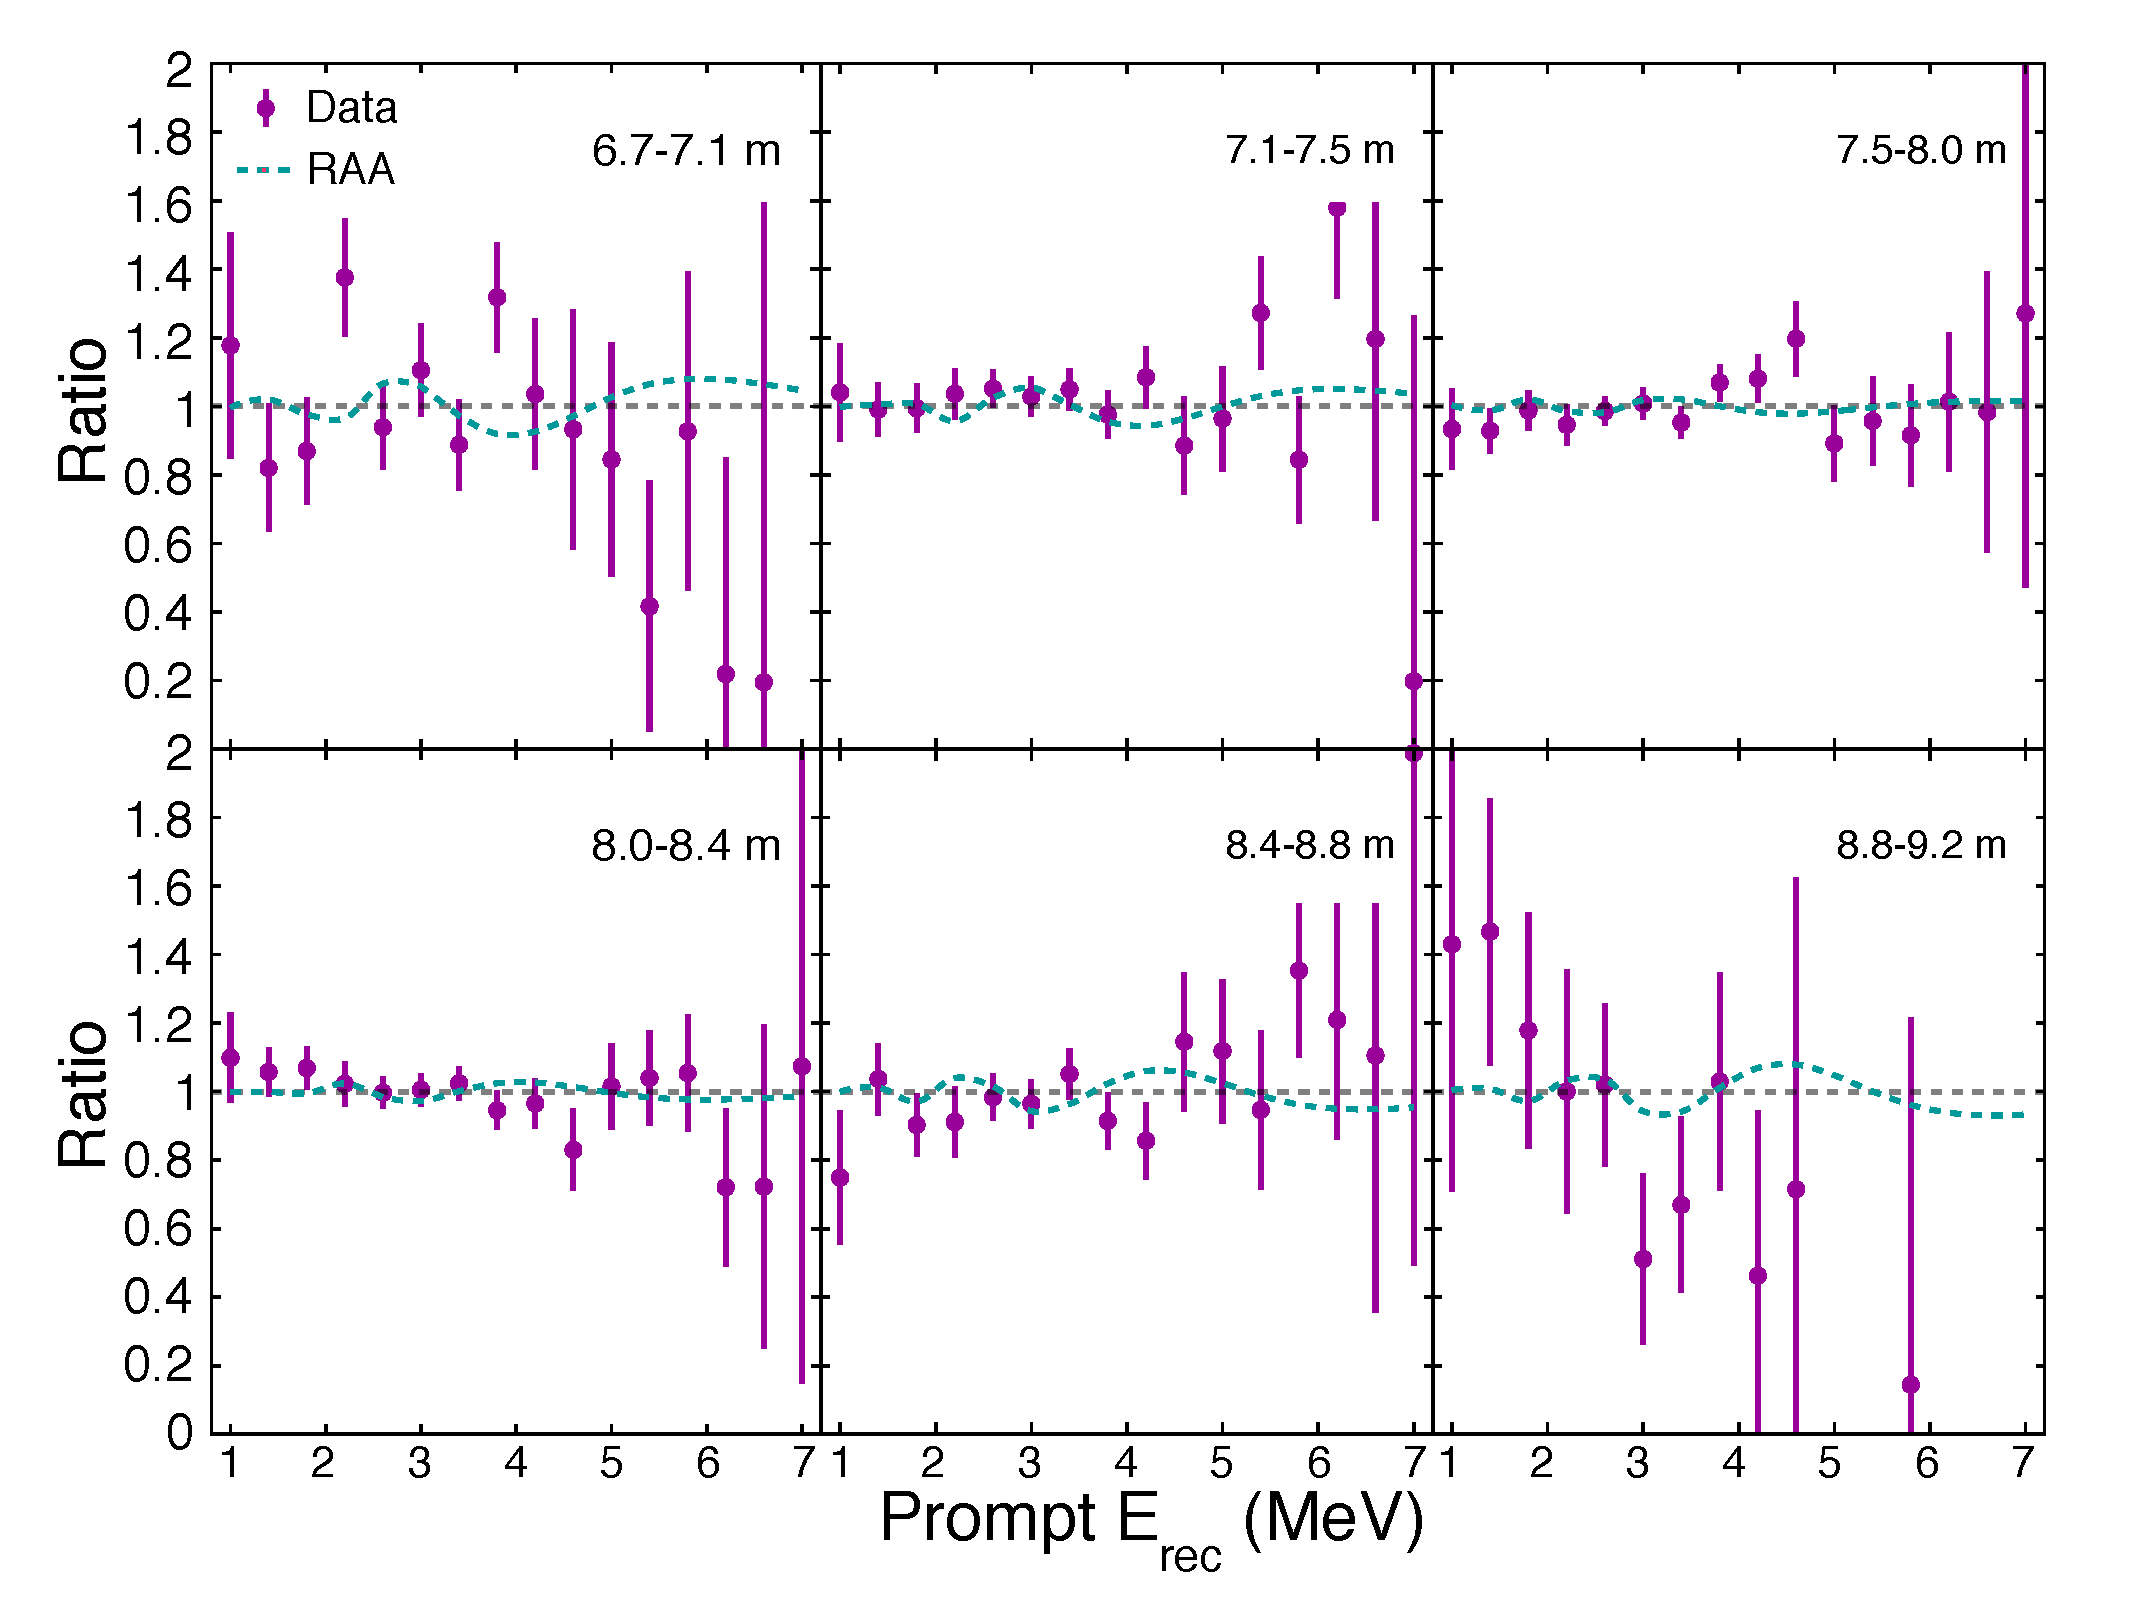
\includegraphics[width=0.7\linewidth]{tex/7-oscillation-images/BaselineSpectra}
	\caption{}
	\label{fig:baselinespectra}
\end{figure}

\begin{figure}[H]
	\centering
	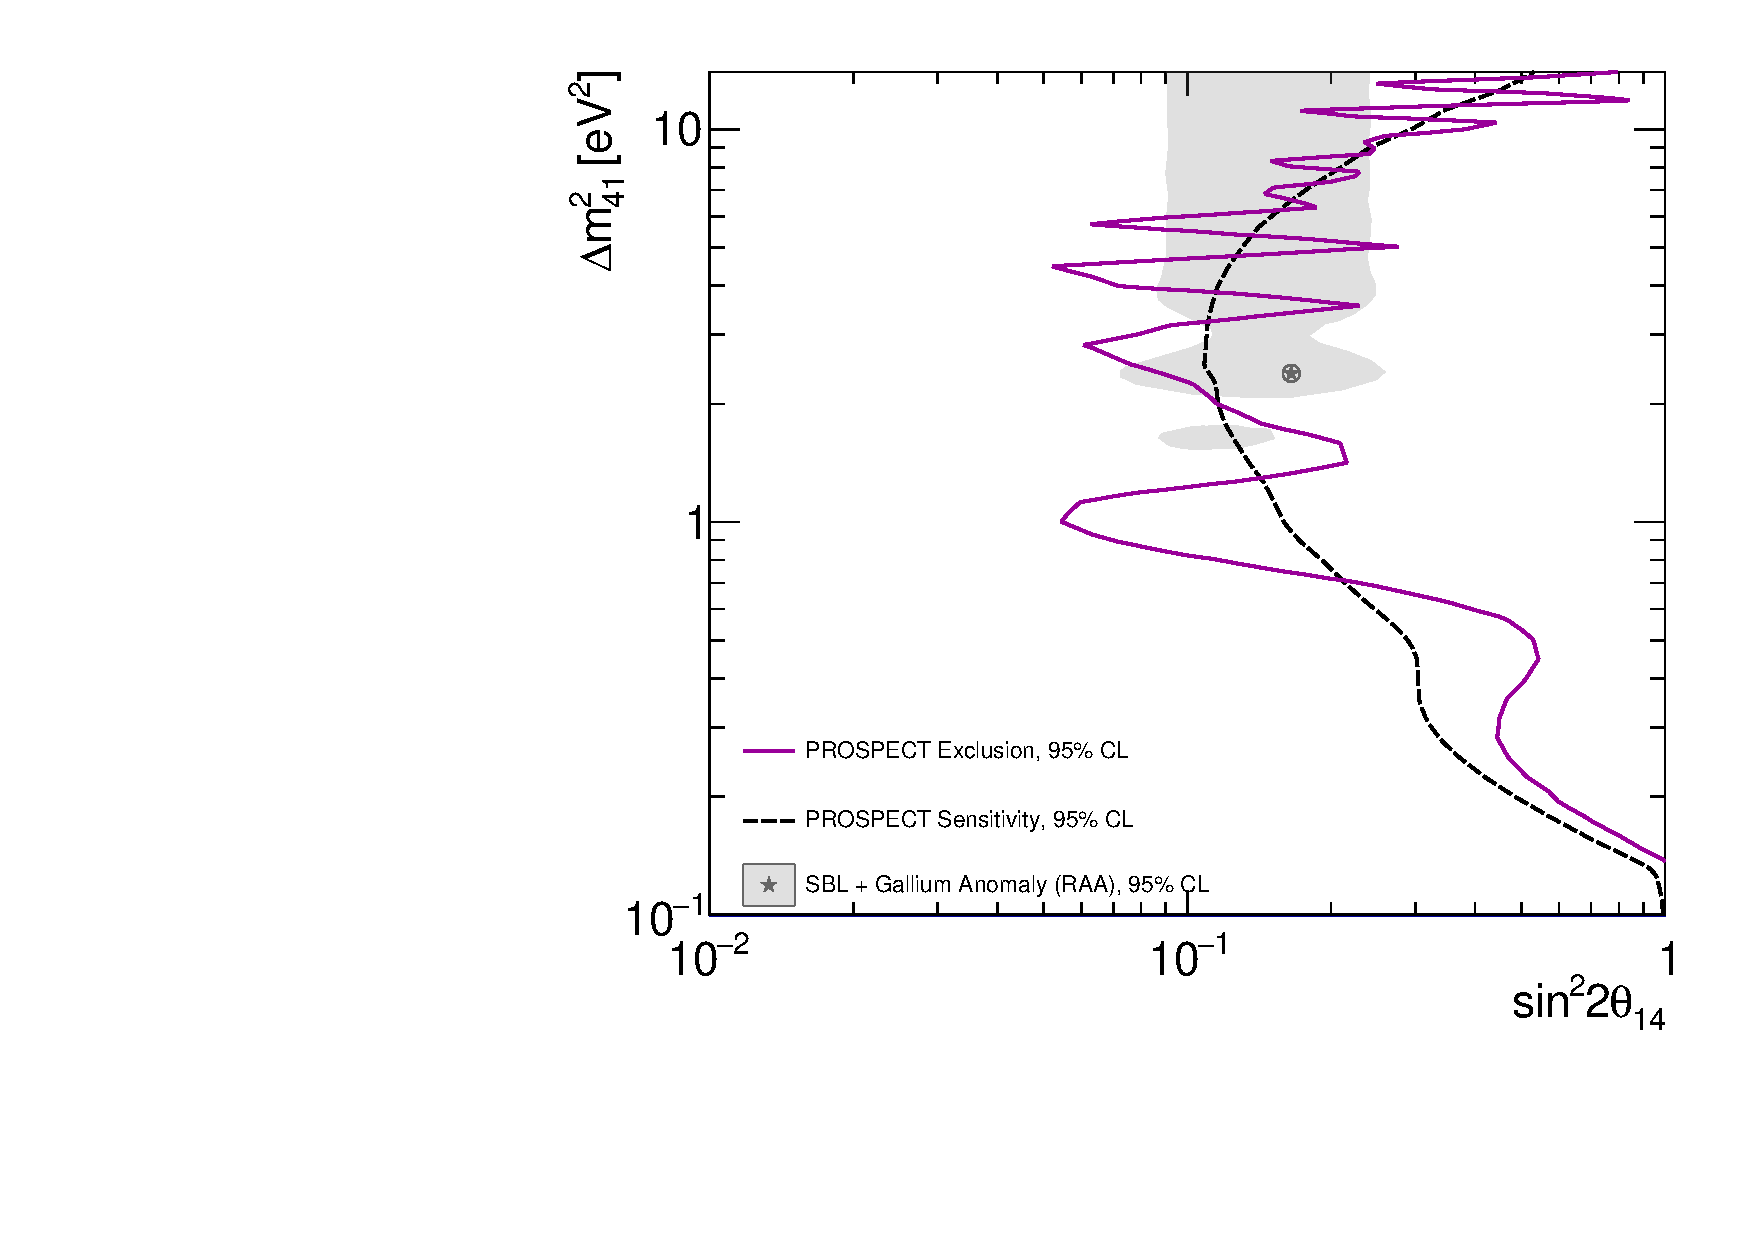
\includegraphics[width=0.7\linewidth]{tex/7-oscillation-images/Exclusion_Sensitivity_Final}
	\caption{}
	\label{fig:exclusionsensitivityfinal}
\end{figure}



\section{Spectrum Results}
\begin{figure}[H]
	\centering
	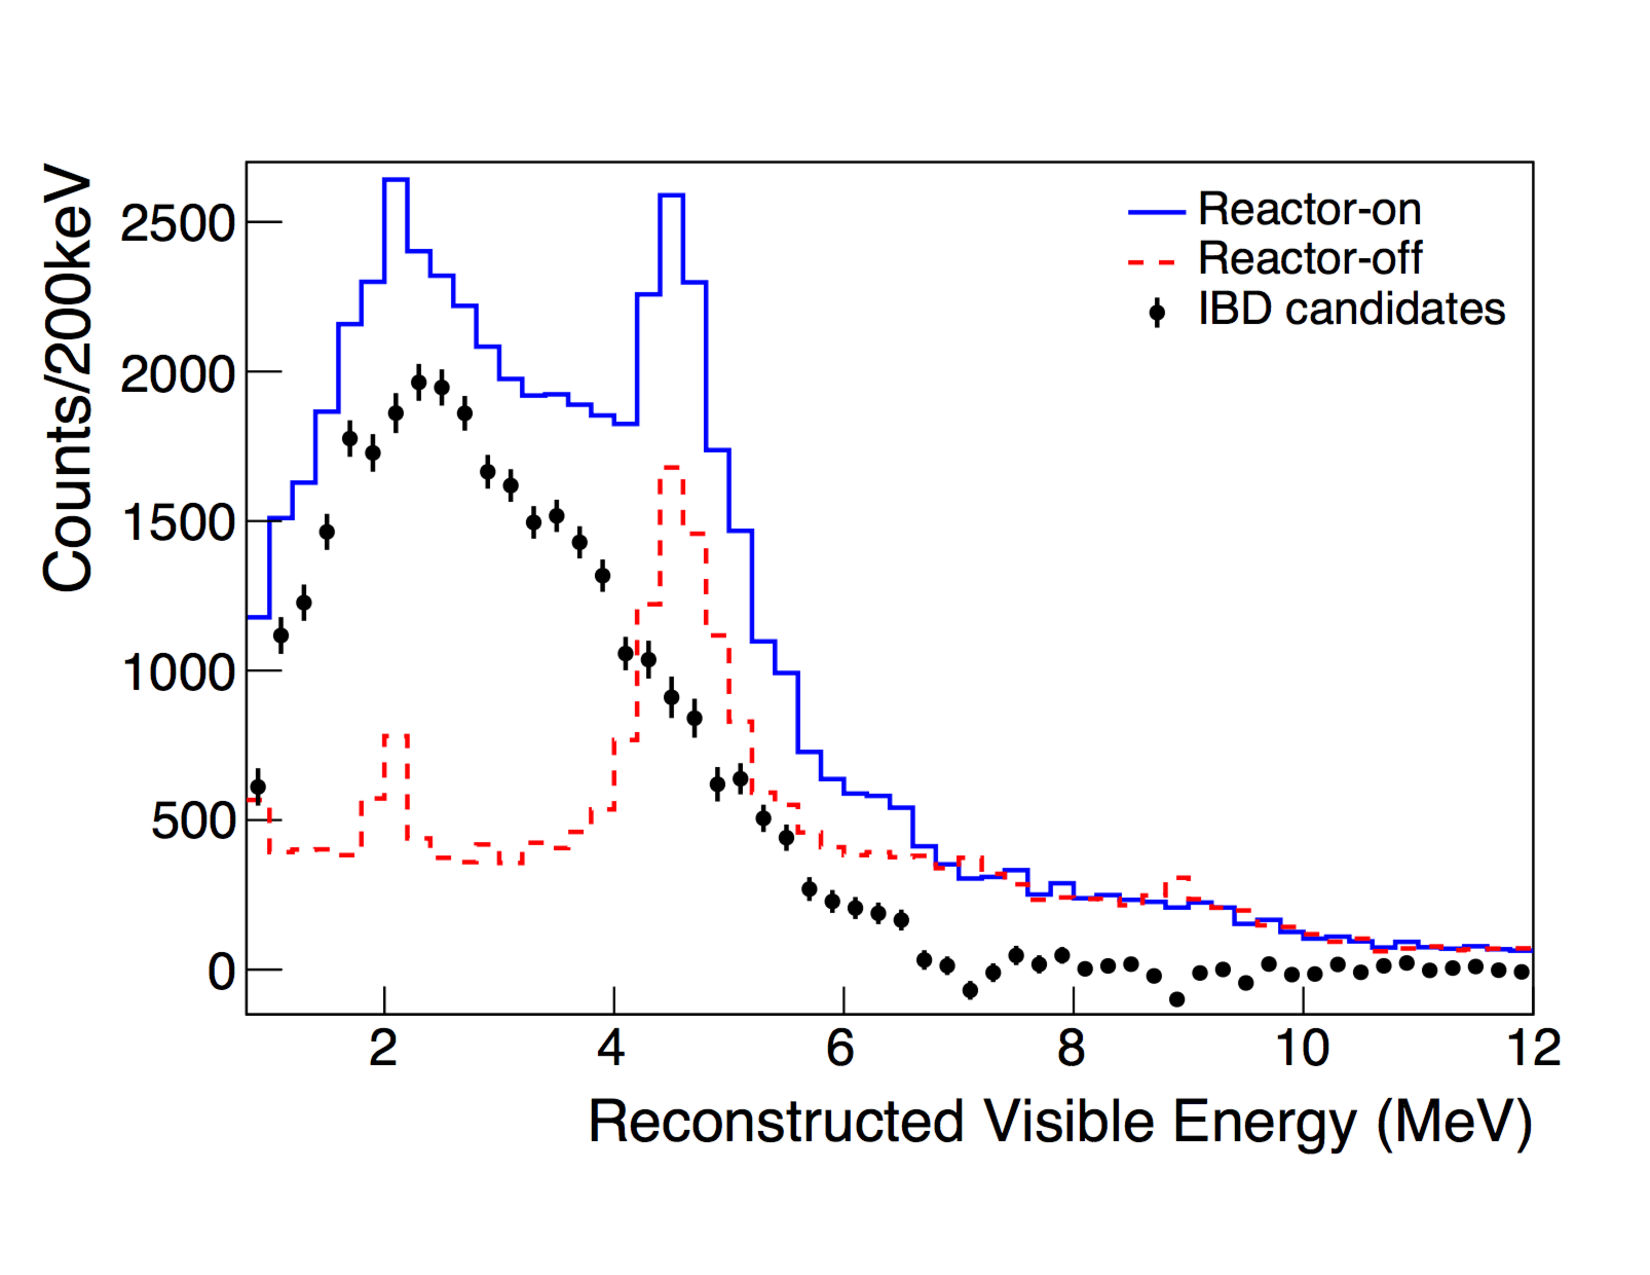
\includegraphics[width=0.7\linewidth]{tex/7-oscillation-images/Spectrum}
	\caption{}
	\label{fig:spectrumresults}
\end{figure}



